\chapter{Design \& Model}
\label{chap:model}

We now present our design and model for mixed-criticality scheduling support in a high-assurance
system such as \selfour. 

Our goal is to provide support in the kernel for mixed-criticality workloads.  This involves
supporting tasks of different real-time strictness (\gls{HRT}, \gls{SRT}, best effort), different
criticalities, and different levels of security.  Such tasks should not be forced into total
isolation, but be permitted to share resources without violating their temporal correctness
properties through mechanisms provided by the kernel.

To achieve this we require temporal isolation: a feature of resource kernels, whose mechanisms we
apply to our research platform, \selfour.  However temporal isolation is not enough: mixed-criticality
systems require asymmetric protection rather than temporal isolation, as a result we leverage
traditional resource kernel reservations but decouple them from priority, allowing the processor to
be overcommitted while providing guarantees for the highest priority tasks.

In this section we first address how we integrate resource kernel mechanisms with \selfour with
mechanisms for temporal isolation. We then explain
priority decoupling and our model for temporal isolation in shared resources, with clients of
different criticalities, temporal sensitivity, and trust.

Our design goals are as follows:
\begin{description}\sloppy
    \item[Capability-controlled enforcement of time limits:] In general, capabilities
      help to reason about access rights. Furthermore, they allow a
        seamless integration with the existing capability-based spatial
          access control of security-oriented systems such as \selfour.
    \item[Policy freedom:] In line with microkernel philosophy
        \citep{Heiser_Elphinstone_16}, the model should not force systems
        into a particular resource-management policy. In particular, it
        should support a wide range of scheduling policies and
        resource-sharing models, such as locking protocols.
i%    \item[Explicit notion of criticality] that is separate from priority /
 %                   time sensitivity.
    \item[Efficient:] The model should add minimal overhead over the best
                      existing implementations. In particular, it should be compatible
                        with fast IPC implementations in high-performance microkernels.

    \item[Asymmetric Protection:] The model should allow for asymmetric protection, where high
        criticality tasks can disrupt low criticality tasks.
    \item[Safe resource sharing:] mechanisms for sharing between applications of time sensitivity
        and criticality.
\end{description}

The model  provides temporal isolation mechanisms from the kernel, while allowing for more complex
scheduling policies to be implemented at user level.

\section{Scheduling}

We outlined four core resource kernel mechanisms -- admission, scheduling, enforcement and
accounting -- that are essential to resource kernels for implementing temporal isolation.  However,
as noted in \Cref{sec:resource-kernels}, such kernels are monolithic, where all policy, drivers and
mechanisms are provided by the kernel.

Microkernels like \selfour offer a different design philosophy, based on the principle of
minimality~\citep{Liedtke_95}, where mechanisms are only included in the kernel if they would
otherwise prevent the implementation of a systems required functionality.  Existing literature is
divided as to whether resource kernel mechanisms should be provided by the kernel or at user-level.

The goals of resource kernels do not directly align with that of microkernels in general.  This is
because microkernels do not directly manage all resources in the system, but provide mechanisms for
the system designer to implement custom resource management policies.  In fact, in the context of a
microvisor, the resource managers may actually be OS guests.

In \selfour, mechanisms for physical memory, device memory, interrupt and \IO port management are
exposed to the user via the capability system, as outlined in \cref{chap:sel4}. As a result, the
only resource that the kernel needs to provide reservations for is processing time.  We now examine
how each of the four resource kernel mechanisms are implemented in our model.

\subsection{Scheduling algorithm}

Our model retains a scheduler in the kernel, and that scheduler is fixed-priority, as per previous
incarnations of L4. 
The kernel will not adjust priorities on its own, but they can be changed with a
system call. 
The scheduling algorithm also remains with priority determining what is scheduled next, \ie the
highest-priority runnable (not blocked) thread.

\subsubsection{Kernel scheduling}

We retain the scheduler in the kernel, unlike \composite, for two reasons: to maintain a small
trusted computing base, and for performance. Any system with multiple threads of execution, which is
required in a mixed-criticality system, must have a scheduler, which for the purposes of temporal isolation 
is part of the trusted computing base. If a system must have a scheduler, and in a mixed-criticality
system, with untrusted components, that scheduler must be in a separate protection domain to those
untrusted components, then a scheduling decision will require at least two context switches: from
the preempted thread to the scheduler, and from the scheduler to the chosen thread. Placing a basic
scheduler in the kernel reduces this overhead. 

Additionally, as the scheduler is a core component of the system it must be verified: by keeping the
scheduler in the kernel we maintain the current verification. Verification of a user level scheduler
and its interaction with the kernel is a far more complex task, especially as verification of
concurrent systems is very much an open research challenge. 

One might claim maintaining a scheduler in the kernel is a violation of our goal of policy freedom.
However we maintain this is not the case, which comes down to our choice of fixed priorities over
\gls{EDF}.

\subsubsection{Fixed priorities}

We choose \gls{FP} over \gls{EDF} for three reasons; 
fixed-priority is dominant in industry
as shown in \cref{chap:operating-systems} and maps well to \gls{FP} with \gls{RM} priority assignment; and dynamic scheduling policies like
\gls{EDF} can be implemented at user level; and \gls{FP} has defined behaviour on overcommitted
systems.

Real-time literature is utterly divided between which real-time scheduling algorithm should be
deployed as the core of real-time systems, \gls{EDF} or \gls{FP}.  In the systems community,
\gls{FP} is far more dominant due to its inclusion in \gls{POSIX} and its compatibility with
existing, priority-based best effort systems.  Support for \gls{FP} is important as it is most
prevalent in industry.  
However the opposite is not true: mapping the dynamic priorities of EDF to a fixed-priority
is non-trivial and would come with high overheads. 
Our approach is consistent with existing designs in Linux  and ADA\citep{Burns_Wellings:crtpa}, which
support both scheduling algorithms, usually with \gls{EDF} at a specific priority.

Therefore our model uses \gls{FP} scheduling as remain a core part of the kernel.  \gls{EDF}
scheduling can be implemented by using a single priority for EDF's dynamic priorities, as we
demonstrate in \cref{s:edf-impl}.

We do not consider Pfair scheduling (recall \cref{s:pfair}) an option, as its high interrupt
overheads and fairness properties are not suitable for hard real-time systems.  Again however, it is
possible to implement a Pfair scheduler at user level.

Our approach is a hybrid of that taken by \composite compared to resource kernels. We provide
mechanisms for user-level scheduling, but also provide a basic scheduler suitable for many
applications. 

The final reason to base the approach on fixed priorities is the ability
to reason about the behaviour of an
overcommitted system. Overcommitting, is important for achieving high
actual system utilisation, given the large time buffers required by
critical hard real-time threads. It is also core to keeping the kernel
policy-free: The degree and nature of overcommitment is a core policy
of a particular system. For example, the policy might require that the
total utilisation of all \crit{high} threads is below the RMS
schedulability limit of 69\%, while \crit{low} threads can overcommit,
and the degree of overcommitment may depend on the mix of hard RT,
soft RT and best-effort threads. Such policy should be defined and
implemented at user level rather than in the kernel.

As indicated in \autoref{s:theory}, the result of overcommitting in an
EDF-based system is hard to predict, and such a system is hard to
analyse. In contrast, with fixed priority the result is easy to
understand: If the sum of utilisations of threads at priority \(\geq
P\) is below the utilisation bound, then all those threads will meet
their deadlines, while any thread with priority \(<P\) may miss. This
allows easy analysis of schedulability, including when the system
criticality changes.

\subsection{Scheduling contexts}
\label{s:scs}

At the core of the model is the \emph{\gls{SC}} as the
fundamental abstraction for time allocation, and the basis of 
the enforcement and accounting mechanisms in our model.
An \gls{SC} is a representation
of a reservation in the object-capability system, which means that 
are first-class objects, like threads, address spaces, or
communication endpoints (ports). An SC is represented by a capability to a
scheduling context object (scCap).

An scCap represents the privilege to access the processor, i.e.\ a
time capability. In order to run, a thread needs an scCap, which represents the
maximum CPU bandwidth the thread can consume.
In a multicore system, an SC represents the right to access a
particular core. Core migration, e.g.\ for load balancing, is policy
that should not be imposed by the kernel but implemented at user
level. A thread is migrated by replacing its SC with one tied to a
different core. This renders the kernel scheduler a partitioned scheduler, 
which aligns with our efficiency goal; partitioned schedulers outperform global
schedulers~\citep{Brandenburg_PHD}.

The unfungible nature of time in real-time systems requires that the
bandwidth limit must be enforced within a certain time window. We
achieve this by representing an SC by a \emph{period}, \(T\), and a
\emph{budget}, \(C\), where \(C\leq T\) is the maximum amount of time
the SC allows to be consumed in the period. \(U=\frac{C}{T}\) represents the
maximum \emph{CPU utilisation} the SC allows. The SC can be viewed as
a generalisation of the concept of a time slice that is used on many
systems (including present mainline \selfour).

In order to support MCS, we do not
change the meaning of priority, but what it means for a thread to be
\emph{runnable}: We associate each thread with a SC, and
make it non-runnable if it has exhausted its budget. 


\glspl{SC} can be gracefully integrated into the 
existing model used in \selfour,
logically replacing the time slice attribute with the scCap. 

Unlike Fiasco's scheduling contexts~\citep{Lackorzynski_WVH_12}, which
are superficially similar to ours, we retain priorities as a thread
attribute rather than making them part of SCs.\footnote{Fiasco's scheduling
contexts were developed for an old API version that was not
capability-based, and it is not obvious how they would integrate
with the capability system of present Fiasco.OC.} The advantage of keeping the two
orthogonal will become evident in \autoref{s:locking}.

\subsection{Accounting}

We introduce a new invariant that the currently running thread must have a scheduling context 
with available budget. Any time executed on a processor is billed to the current threads scheduling
context.

We account for processing time using processor cycles, as opposed to fixed time ticks, as discussed
in \cref{s:tick-v-tickless}. A tickless model offers less overheads and more precision to real-time 
tasks, which suffer \gls{WCET} penalties for every preemption. Additionally, the evaluation will
show in \cref{s:eval-timer}, the cost of reprogramming a timer has significantly decreased on modern hardware. 

\subsection{Enforcement}

Our model offers two options for enforcement: threads can have an optional timeout fault handler,
which results in a fault being delivered should that thread exhaust its budget. Otherwise the kernel
will not schedule threads until their budget is replenished. 

\subsection{Admission control}
\label{sec:model-admission}

Setting budgets is admission control and requires appropriate
privilege. The total available time on a core is represented in a
(virtual) per-core scheduling-control capability, \code{sched\_control}.
Access to this capability, provides the admission-control
privilege. This is analogous to how \selfour controls the right
to receive interrupts, which is controlled by the IRQ\_control
capability as introduced in \cref{s:capabilities}. Like time, IRQ sources are non-fungible.

Unlike the reservations in resource kernels, the scheduling context does not 
act as a lower-bound on CPU bandwidth that a thread can consume. This, combined with the
user-level admission control, is also key to allowing system designers to over-commit the system. 

By designating admission tests as user-level policy, we allow system designers complete freedom
in determining which admission test to use, if at all, and when that test should be done.
Consequently, they can be run dynamically at run-time, or offline, as per user-level policy.

Thus, the kernel places no restriction on the creation of reservations apart from minor validity
checks (\ie $C \leq T$).
For example, some high-assurance systems may sacrifice utilisation for safety with a very basic but easily verifiable, online, admission test.
Other implementations may conduct complex admission tests offline in order to obtain the highest possible utilisation, using algorithms that are not feasible at run time.
Some systems may require dynamic admission tests that sacrifice utilisation or have increased risk.
Basic systems may require a simple break up of the processing time into rate-limited reservations.
By taking the admission test out of the kernel, all of these extremes (and hybrids of) are optional policy for the user.

A consequence of this design is that more reservations can be made than processing time available.
This is a desirable feature: it allows system designers to overcommit the system, while features of the scheduling mechanisms provided by the kernel guarantee that the most important tasks get their allocations, if the priorities of the system are set correctly.

However, allowing any thread in the system to create reservations could result in overload behaviour and violation of temporal isolation.
To prevent this, admission control is currently restricted to the task that holds the scheduling
control capability for each processing core.

\subsection{Replenishment}

Scheduling contexts can be \emph{full} or \emph{partial}. A thread with a \emph{full} SC, where
\(C=T\), may monopolise whatever
CPU bandwidth is left over from higher-priority threads, while high-priority threads with full
\glspl{SC} may monopolise the entire system. 
Partial \glspl{SC}, where \(C<T\), are not runnable once
they have used up their budget, until it is replenished, and form our mechanism for temporal
isolation.  

Full \glspl{SC} are key to maintaining policy freedom and performance; while systems
must be able to use our mechanisms to enforce upper bounds on execution, the usage of 
those mechanisms is policy. If a task is truly trusted, no enforcement is required,
as in standard \gls{HRT} systems. They can also be used for best-effort threads which run in slack time.
The \(C\) of a full \gls{SC} represents the timeslice, which once expires results in round robin
scheduling at that priority. 

From a performance perspective full \glspl{SC} prevent mandatory preemption overheads 
that derive from forcing all threads in a system to have a reservation. Threads with a full
budget incur no inherent overhead other than the preemption rate $1/T$.

Threads with \emph{partial} \glspl{SC} have a limited budget, which forms an upper
bound on their execution. For replenishment we
use the sporadic servers model as described in \cref{p:sporadic} with an
implementation based on the algorithms presented
by~\citet{Stanovic_BWH_10}. 

The combination of full and partial \glspl{SC}  and the ability to overcommit distinguishes our
model from that of resource kernels. However, a full resource kernel should be able to be
constructed on top of the mechanisms our model provides.

\subsubsection{Sporadic servers}

We use sporadic servers as they provide a mechanism for isolation without requiring the kernel
to have access to all threads in the system, unlike other approaches discussed in
\cref{background:fp-isolation}, \eg  priority exchange servers and slack stealing.
Deferrable servers do not require global state but are avoided due to the back-to-back
problem. 

Recall that sporadic servers work by preserving the
\emph{sliding window} constraint, meaning that during any time
interval not exceeding the period, no more than $C$ can be consumed.
This stops a thread from saving budget until near the end of its
period, and then running uninterrupted for more than $C$. It is achieved by tracking any leftover
budget when
a thread is preempted at time \(t\), and scheduling a replenishment for time  $t+T$.

In practice we cannot track an infinite number of
replenishments, so in a real implementation, once the number of
queued replenishments exceeds a threshold, any excess budget is
discarded. If the threshold is one, the behaviour degrades to polling
servers~\citep{Sprunt_SL_89a} where any unused budget is lost and the
thread cannot run until the start of the next period.

There is an obvious cost to replenishment fragmentation that will
arise from preemptions, and polling servers are more efficient in the
case of frequent preemption \citep{Li_WCM_14}; an arbitrarily high
threshold makes little sense. The optimal value depends on
implementation details of the system, as well as the characteristics
of the underlying hardware.
We therefore make the threshold an attribute of the SC. \glspl{SC} are variably sized,
such that system designers can set this bound per SC. This is a generalisation of the approach used
in Quest-V~\citep{Danish_LW_11}, where \IO reservations are polling servers and other reservations 
are sporadic servers, as policy which can easily be implemented at user-level with variably sized
\glspl{SC}.

\subsection{Budget overrun}\label{s:timeout}

Threads may exhaust their budgets for different reasons. A budget may
be used to rate-limit a best-effort thread, in which case budget
overrun is not different to normal time-slice preemption of
best-effort systems. A budget can be used to force an untrusted thread
to adhere to its declared WCET. Such an overrun is a contract violation, which may be reason
to suspend the thread or restart its subsystem. Finally, an overrun by
a critical thread can indicate an emergency situation; for example,
critical threads may be scheduled with an optimistic budget to provide
better service to less critical threads, and overrun may require
provision of an emergency budget or a system-criticality change.

Clearly, the handling of overrun is a system-specific policy, and the
kernel should only provide appropriate
mechanisms for implementing the desired policy. Our core mechanism is
the \emph{timeout exception}, which is raised when a thread is
preempted. To allow the system to handle the exceptions, each thread
is optionally associated with a timeout exception handler, which is
the temporal equivalent to a (spatial) protection exception. When a
thread is preempted, the kernel notifies its handler via an IPC message. The
exception is ignored when the thread has no timeout exception handler, and the thread
can continue to run once its budget is replenished.

Similar to a page fault handler, timeout fault handlers can be used to adjust thread parameters dynamically as may be required for a \gls{SRT} system, or raise an error.
The handler has a choice of a range of overrun policies, including:
\begin{itemize}
      \item providing a one-off (emergency) budget to the thread and letting it continue,
       \item permanently increasing the budget in the thread's SC,
       \item killing/suspending the thread, and
       \item changing the system criticality level.
       \end{itemize}
Obviously, these are all subject to the handler having sufficient
authority (\eg \code{sched\_control}.

If a replenishment is ready at the time the budget expires, the thread
is immediately runnable. It is inserted at the end of the ready queue
for its priority, meaning that within a priority, scheduling of
runnable threads is round-robin.

\subsection{Priority assignment}

Assignment of priorities to threads is user-level policy. One approach is to simply use
rate-monotonic scheduling: where priorities are assigned to threads based on their period, and
threads use scheduling contexts that match their sporadic task parameters.  Each thread in the
system will be temporally isolated as the kernel will not permit them to exceed the processing time
reservation that the scheduling context represents.

However, the system we have designed offers far options than simple rate-monotonic fixed-priority
scheduling.  Policy freedom is retained as reservations simply grant a potential right to processing
time, at a particular priority.  What reservations actually represent is an upper bound on
processing time for a particular thread.  Low priorities threads are \emph{not} guaranteed to run if
reservations at higher priorities use all available CPU.  However, threads with reservations at low
priorities will run in the system slack time, which occurs when threads do not use their entire
reservation.

The implication is that a system could use a high range of priorities for rate-monotonic threads,
while best-effort and rate-limited threads run at lower priorities.  Another alternative is to have
real-time threads running at the EDF-priority, where they will be temporally contained, with
non-real time threads running at lower priorities.  Many other combinations are possible.

\subsection{Asymmetric Protection}

Recall that in a mixed-criticality system, asymmetric protection means that tasks with higher
criticality can cause deadline misses in lower criticality tasks.  Two approaches to mixed
criticality scheduling that provide asymmetric are slack scheduling and
\gls{RTA}\citet{Burns_Davis_14}.

Under slack scheduling, low-criticality tasks run in slack time of high criticality tasks.  Our
model supports this easily: hi criticality tasks are given reservations to all of processing time at
high priorities, and low criticality tasks given reservations at a lower priority band.

\gls{RTA} relies on suspending low criticality tasks if a high criticality task runs for longer than
expected.  In general, \gls{RTA} schemes involve two system modes: a \crit{HI} mode and a \crit{LO}
mode.  In \crit{LO} mode, high criticality tasks run with smaller reservations, and the remaining
CPU time is used for low criticality tasks.  If a high criticality task does not complete before its
\crit{LO} mode reservation is exhausted, the system switches to \crit{HI} mode: all low criticality
tasks are suspended.  This is also supported by our model: a high priority scheduling thread can be
set up to receive temporal faults when a task does not complete before its budget expires.  On a
temporal fault, the scheduling thread can extend the reservation of the high priority task and
suspend all low priority tasks.

\subsection{Summary}

The scheduling, accounting and enforcement mechanisms presented are sufficient to support temporally
isolated, fixed-priority or \gls{EDF} scheduled real-time threads. By keeping admission control
out of the kernel we preserve policy freedom, while the mechanisms provided allow for a full
resource kernel to be built, or other types of system which require the ability to over-commit.
Additionally, we have maintained
support for best-effort threads, and have added the ability to provide asymmetric protection for
mixed-criticality workloads. 
In the next section, we show how our model provides mechanisms for resource sharing. 

\section{Resource sharing}\label{s:locking}

Bringing mixed-criticality to resource sharing is important for future cyber-physical systems. We 
present our model for resource sharing in terms of the three core mechanisms taken from resource
kernels -- prioritisation, charging and enforcement -- presented in \cref{sec:resource-kernels}.

We consider shared resources as separate threads accessed via synchronous \gls{IPC}, as this
mechanism ultimately means changing which thread is currently running on the processor, and thus
changing where processing time is being spent. Note that we focus our analysis on shared servers
where the server doesn't trust its clients, and the clients do not trust each other. Trusted
scenarios do not require this level of encapsulation: user-level threads packages can implement
locking protocols with libraries such as \texttt{pthreads}.

Access to shared servers encapsulating shared resources requires
cross-address-space IPC. For minimising invocation cost, it is
essential that scheduler invocations are avoided during IPC. This has
historically been done by L4
microkernels~\citep{Heiser_Elphinstone_16}. Not bypassing the
scheduler is the main reason why IPC on most other systems is
significantly slower than that of L4 kernel, e.g.\ at least a factor
of four in CertiKOS~\citep{Gu_SCWKSC_16}.

Past L4 kernels avoided the scheduler by time-slice donation, where a
server could execute on the client's time slice. While fast, this
model is unprincipled and hard, if not impossible, to
analyse. For example, the time slice may expire during the server's
execution, after which the server will run on its own time slice.
This results in no proper accounting of the server's execution, and no temporal isolation, and
relates to the precision problems discuss in \cref{s:tick-v-tickless}.

The proposed model supports shared servers, including scheduler
bypass, in a principled way through \emph{scheduling context
donation}: A client invoking a server can pass its SC along, so the
server executes on the client's SC, until it replies to the
request. This ensures that the time consumed by the server is billed
to the client on whose behalf the servers's work is done.

\subsection{Scenarios}

Our analysis of is guided by two models for the flow of time between communicating threads in a
system: a client-server or \gls{RPC} scenario, and a data-flow scenario.

\subsubsection{Client-Server}

The client-server scenario involves clients contacting servers in an \gls{RPC} style fashion: the
client sends a message to the server, the server executes an operation on the clients behalf and
replies.  Servers can be clients too: a server may make a nested request to another server on behalf
of a client.  There can be multiple servers, and multiple clients in operation at the same time.

An example of this scenario is illustrated in \Cref{fig:client-server}, albeit with just one client
and nested servers. The figure shows both stages of \gls{IPC} illustrated earlier in \cref{f:ipc} as
one. 

\begin{figure}
    \centering
    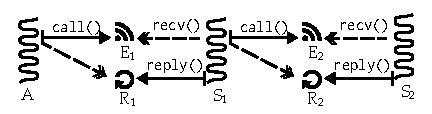
\includegraphics[width=\textwidth]{client-server1}
      \caption{Nested client-server \gls{RPC} scenario, using the legend presented in \cref{f:legend-1}.}
      \label{fig:client-server}
\end{figure}

\subsubsection{Data-flow}

In the data-flow scenario, as illustrated in \Cref{fig:dataflow}, an external event triggers the
release of a job.  The job passes through a chain of activities, all doing different forms of
processing.  Only one job can be active in an activity at a time, and the next job cannot be
released until the previous has finished (consistent with the sporadic task model).  Forks are
permitted in the chain, although the forks must be choices: one job cannot trigger two jobs, as a
processor reservation cannot be transferred to two jobs at once.  Cycles and sequences are permitted
in the chain.

\begin{figure}
      \centering
      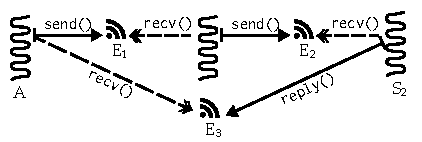
\includegraphics[width=\textwidth]{dataflow1}
      \caption{Data-flow scenario, using the legend presented in \cref{f:legend1}.}
      \label{fig:dataflow}
\end{figure}

Both scenarios can be combined to form a larger system.

\subsection{Prioritisation}

We indicated in \Cref{s:scs} that scheduling contexts are separate from thread control blocks in
order to support resource sharing. Additionally, unlike previous microkernel designs for \glspl{SC}, priority
remains an attribute of the execution context. By doing so, \gls{PIP} is not the default protocol
enforced by the kernel. 

\gls{HLP} maps neatly to this model: if server threads are assigned the ceiling protocol of all of
their clients, then when the \gls{IPC} rendezvous occurs and we switch from client to server, the
servers priority is used.

The choice of \gls{HLP} is intentional: if the scheduling context holds the priority, then \gls{PIP}
is forced by the mechanism. Since \gls{PIP} has a known high preemption overhead, this would violate
our criteria of policy freedom and efficiency.  
\gls{PCP} is not an option for another reason; the protocol requires the kernel to maintain shared
state about all resources and threads to reason about priority, which is not compatible with the
\gls{IPC} and endpoint model. % TODO why

However \gls{PIP} and \gls{PCP} can used with this mechanism albeit in a more complex fashion, by
proxying requests to shared resources via a scheduling server which manipulates the priorities
appropriately. For \gls{PIP}, only one server per resource would be required and could exist in the
same address space as the resource. Since \gls{PCP} requires global state, an implementation would
require a shared service for all threads sharing a set of resources.

\subsection{Charging}

Unlike prior implementations of scheduling contexts discussed in \cref{s:sc-intro},
donation is not compulsory, which provides more policy freedom than prior models.

% TODO up to here
Another distinguishing factor of scheduling context donation in our mode


Passive servers effectively provide a migrating-thread
model~\citep{Ford_Lepreau_94, Gabber_SBBS_99}, but without requiring
the kernel to manage stacks. They also
provide a simple, and essentially free, implementation
of IPCP: The server is configured with
the ceiling priority of its clients, making its execution atomic with
respect to all clients. This is possible thanks to decoupling SCs from
priorities. The main drawback of IPCP, namely the requirement that all
lockers' priorities are known \emph{a priori}, is easy to enforce in a
capability-based system: The server can only be accessed through an
appropriate invocation capability, and it is up to the system designer
to ensure that such a capability can only go to a thread whose
priority is known or appropriately controlled.

If a passive server exhausts its budget, it and any waiting clients
are blocked until the budget is replenished. On its own, this means that a client
not only has to trust its server, but all the server's other
clients. This would rule out sharing a server between clients of
different criticality.

Timeout exceptions can be used to remove this need for trust, and
allow a server to be shared across criticalities. The
server's timeout handler can, for example, provide an emergency budget
to continue the operation (useful for \crit{high} clients) or abort
the operation and reset or roll back the server. The latter option is
attractive for minimising the amount of budget that must be reserved
for such cases.

A server running out of budget constitutes a protocol violation
by the client, and it makes sense to penalise that
client by aborting. Helping schemes, such as PIP or bandwidth
inheritance, as implemented in Fiasco,
make the waiting client pay for
another client's contract violation. This not only weakens temporal isolation,
it also implies that the size of the required reserve budget
must be server's full WCET. This places a restriction on the server
that no client request exceed a blocking time that can be tolerated by
all clients, or that all clients must budget for the full server WCET in
addition to the time the server needs for serving their own request.
Our model provides more flexibility: a server can use a timeout
exception to finish a request early (e.g.\ by aborting), meaning that clients can only be
blocked for the largest budget of the other clients (plus the short
cleanup time).

Where desired, helping schemes can be implemented on top of our
model, e.g.\ by using a gateway server that adjusts priorities as
requests come in.




\subsection{Resource sharing models}

We consider three existing models for resource sharing over IPC: reservation-per-thread, timeslice donation, and migrating threads.
In all models, the shared server or phase is assumed to have a known \gls{WCET}, which should match that of the strictness real-time task using the server.

\subsubsection{Reservation-per-thread}
\label{sec:reservation-per-thread}

In the reservation-per-thread model, reservations are assigned to every thread in the system, clients and servers alike.
Server budgets must be sufficient to serve all clients or the system will be bottle-necked on the server.
In order to calculate sufficient budgets, the number of client requests must be known \emph{a priori}.

This design does not provide temporal isolation, as the server executes on its own budget.
If one client launches a denial of service attack on the server, depleting the servers budget, then other clients are starved.
Servers could be placed at a higher priority with a 100\% CPU reservation, but this is also problematic as the server can then monopolise the entire system in the case of rogue clients.

While our resource sharing mechanisms should not rule out this policy, it is only suitable for systems where all clients are trusted and the amount of requests each client makes is known \emph{a priori}, or systems that have lax temporal requirements.

\subsubsection{Timeslice donation}

Fiasco.O.C~\citep{Steinberg_BK_10} implements timeslice donation, where servers run on the reservation of the client, at the priority of the client.
%TODO define active
Such a design allows for temporal isolation as clients can only make requests while their reservation is active, and servers deplete the clients reservation.

As the server inherits the clients priority, this design has the same preemption overheads \gls{PIP}, discussed in \Cref{sec:priority-inheritance}.
Implementing priority inheritance requires the kernel to track dependencies between servers and clients, which requires a large amount of book keeping.

Further challenges arise if the clients reservation expires while the server is still executing.
Without further mechanisms, the resulting scenario leaves the server unable to service other clients, as it is in the middle of serving another clients request.

In the context of a hard real-time system, expiry will not occur, as client reservations are based on \gls{WCET}.
However, systems that support other real-time models -- soft real time and rate based tasks --  must solve the issue.
In Fiasco.O.C expiry is ameliorated by further applying priority inheritance, which the authors refer to as \emph{helping}.
If a server is stuck servicing a request, and a second client attempts to make a request of the server, the server will finish the previous clients request on the second clients budget and priority.

Dependency tracking in this model quickly becomes very complex when clients and servers use chained requests.
Additionally, because priorities must be returned to clients, this model does not support the data-flow scenario outlined earlier.

\subsubsection{Migrating threads}

\composite~\citep{Parmer_10} takes a different approach to solving the resource sharing model, by using migrating threads (also termed stack-migrating IPC).
On every IPC, client execution contexts (and CPU reservation) transfer to a new stack running in the servers protection domain, resulting in multi-threaded servers.

To implement migrating threads, \composite requires that every server have a mechanism for allocating stacks.
If no memory is available to allocate stacks then the request is blocked.
This solution forces servers to be multi-threaded, and does not solve the problem of a clients budget expiring while the server is in a critical section, which is solved by providing atomic primitives that call the kernel.

We perceive the migrating thread model as valid for systems suited to multi-threaded servers, but do not think it is suitable for microkernel mechanisms to require multi-threaded servers.
Like the reservation-per-thread model, we choose to support this approach, but not enforce it, unlike \composite.

\subsubsection{Summary}

We have outlined reservation-per-thread, timeslice donation and migrating threads.
Our model supports reservations-per-thread and migrating threads, while introducing a design based on timeslice donation without the shortcomings: we remove the need for dependency tracking trees and add support for the data-flow scenario.

\subsection{Scheduling Context Donation}

Finally we present \emph{scheduling context donation}, the new mechanism we have added to the kernel to support resource sharing with temporal isolation.
This model is inspired by timeslice donation, however we utilise \gls{HLP} rather than priority inheritance to reduce preemption and remove the need for a dependency tracking tree.
First we present the basic model, then in the next section we will describe design alternatives for handling budget expiry, which complicates the scenario.

Using \gls{HLP} is not without drawbacks.
Recall that under \gls{HLP} servers run at the ceiling of the priorities of all clients that will access them.
Many claim that such a policy is inappropriate for open systems, as \emph{a priori} knowledge is required of all clients, servers and their priorities in a system.
However, this claim is somewhat unsubstantiated: a system should have a general policy on priorities, especially a system running real-time components.
For example, if a mobile phone operating system allowed all apps to run at the highest priority levels in the system then the phone could be rendered inoperable by apps running at this priority.
Therefore, we believe that is is not unreasonable to deploy \gls{HLP} in our scenario.

Although \gls{PCP} offers greater processor utilisation than \gls{HLP}, we consider its use impractical as it requires too much system state to be drawn into the kernel: the kernel must track a system ceiling and implement priority inheritance.
Using ceilings instead of priority inheritance results in a very clean model when budget expiry is excluded.
Servers inherit the scheduling context of their clients, basically inheriting their budget, while executing on their own priority, resulting in reduced preemption overheads.
When the server replies to clients, the budget is returned.
The kernel has no need to track the dependency relationship, as the reply \gls{IPC} is sufficient to return the scheduling context.
By removing dependency tracking, we can support the data-flow model: instead of replying, a dataflow component simply sends the scheduling context along to the next component.

Unfortunately, scheduling context donation is complicated by budget expiry.
However, since we aim to support rate-based, best-effort and soft real-time threads, budget expiry is required.
The next section will canvas the design options and outline our proposed solutions and mechanisms.

\subsection{Budget Expiry}

In a hard real-time system, we can assume that a client reservations are sufficient to complete requests to servers.
However, in systems with best-effort and soft real-time tasks, no such assumption can be made and client budgets may expire during a server request.
This leaves the server in a state where it cannot take new requests as it is stuck without an active reservation to complete the previous request.
Without a mechanism to handle this event the server, and any potential clients, would be blocked until the client's budget is replenished.

\begin{figure}
    \centering
    \begin{tikzpicture}[node distance=3cm,on grid,>=stealth,very thick]
        \node[state] (a)              {$A_{tcb}$};
        \node[state] (b) [right of=a] {$B_{tcb}$};
        \node[state] (s) [right of=b] {$S_{tcb}$};
    \path[->]
(a) edge [bend left]  node [above] {Call} (s)
(b) edge [bend right] node [below] {Call} (s);
\end{tikzpicture}
\caption{\textbf{Budget expiry:} client A makes a request of server S, but runs out of budget during the request and is blocked. Another client, B, attempts to make a request but finds S blocked.}
\label{fig:budget-expiry}
\end{figure}

\begin{figure}
    \centering
    \begin{tikzpicture}[node distance=3cm,on grid,>=stealth,very thick]
        \node[state] (a)              {$A_{tcb}$};
        \node[state] (b) [right of=a] {$B_{tcb}$};
        \node[state] (s1) [right of=b] {$S1_{tcb}$};
        \node[state] (s2) [right of=s1] {$S2_{tcb}$};
    \path[->]
(a) edge [bend left]  node [above] {Call} (s1)
(b) edge [bend right] node [below] {Call} (s1)
(s1) edge [bend left] node [above] {Call} (s2);
\end{tikzpicture}
\caption{\textbf{Nested budget expiry:} client A makes a request of server S1, which makes a nested request to S1, but runs out of budget during the request and is blocked. Another client, B, attempts to make a request but finds S1 blocked on S2 who has no budget to complete the request.}
\label{fig:nested-budget-expiry}
\end{figure}

\Cref{fig:budget-expiry} illustrates the problem, and \Cref{tab:notation} outlines the notation used.
$A$ makes a request to $S$, such that $A_{sc}$ is donated to $S_{tcb}$.
$A_{sc}$ expires while $S$ is executing $A$'s request.
Then $B$ makes a request to $S$, however $S$ cannot take new requests as it is still still servicing $A$'s request and will not be available until $A_{sc}$ is replenished.

%TODO move
\begin{table}
	\centering
	\begin{tabular}{| c | l |} \hline
    \textbf{Notation} &  \textbf{Meaning}                           \\\hline
       $A$, $B$, $C$, ...   & A task, or user application           \\\hline
	   $S1$, $S2$, $S3$ ... & Resource servers.                     \\\hline
	   $A_{sc}$             & Scheduling context of task A.         \\\hline
	   $A_{tcb}$            & Thread control block of task $A$ \\\hline
	   $A_{b}$              & The budget of task $A$ \\\hline
       $A_{d}$              & Deadline of task $A$                  \\\hline
	   $A_{p}$              & Period of task $A$.                   \\\hline
       $A_{e}$              & The \gls{WCET} of task $A$. \\\hline
     \end{tabular}
	 \caption{Summary of notation used.}
	 \label{tab:notation}
\end{table}

Our goal is to support systems that run best-effort, soft real-time and hard real-time tasks where all tasks can share resources while preserving temporal isolation.
Resource sharing may occur between tasks sharing a real-time model (i.e where all tasks are soft real-time), or between tasks with different real-time models.
In the latter case the resource server must comply with the strictest real-time model of all clients.
This means that for a server that serves hard real-time and soft real-time tasks, the server must have a known \gls{WCET} even though the soft real-time tasks do not.

We outline several potential mechanisms for handling budget expiry: blocking, denying unfeasible requests, emergency reservations for completing requests, rolling back unfinished requests, raising an exception on budget expiry, bandwidth inheritance, and leveraging migrating threads.
Each is analysed according to the following qualities:

\begin{description}
    \item[Schedulable utilisation] The longer the maximum blocking time of each server request, the larger client reservations must be to handle potential blocking. This reduces overall system utilisation, impacting schedulability. What is the impact on schedulability?
    \item[Temporal containment] Tasks sharing a resource cannot be truly temporally isolated, as one task can block the other by simply using the resource. Temporal containment places a limit on the amount of time one task can block another, by bounding the maximum blocking time due to a resource contention. Does the policy offer temporal containment?
	\item[Nested budget expiry] Nested requests (see \Cref{fig:nested-budget-expiry}) is required in both the client-server and data-flow scenarios. Can the policy support expiry in the case of nested requests?
    \item[User-level implications] What changes to user-level applications are required by the mechanism?
    \item[Kernel implementation implications] What changes to the kernel are required by the mechanism.
\end{description}


\subsubsection{Blocking}

Blocking is the default case, where budget expiry is not handled at all and the server is blocked until the clients reservation is replenished.
In the example in \Cref{fig:budget-expiry}, $S_{tcb}$ is blocked until $A_{sc}$ is replenished, and therefore so is $B_{tcb}$.
While clearly not a viable solution we present analysis for the blocking technique as a baseline.

In the best case, if $A_{tcb}$'s request completes when $A_{sc}$ is recharged, then $B$ is only delayed by $A_{p} + S_{e}$.
However, in a pathologically bad (or malicious) case, where $A_{b} \leq S_{e}$, $A_{sc}$ will need to be recharged multiple times before the server request completes.
An upper bound on the delay to other clients caused by one budget expiry is $\frac{S_{e}}{A_{b}} * A_{p}$, which would result in an incredibly pessimistic schedulability test.
If the delay is not factored into the schedulability test, then temporal isolation is violated as $A$ can cause $B$ to miss deadlines.

As far as implementation considerations go, neither the kernel or user-level see any impact as this policy requires no implementation.
Chained invocations only make the schedulability test worse.

\subsubsection{Deny requests}

A simple approach to solving this problem is to deny requests if a client does not have sufficient budget.
The kernel could be configured with the \gls{WCET} of each server and simply deny or post-pone client requests where the budget is insufficient.

This would have a 0 schedulability penalty, but would starve clients and deny requests even if there was no contention for the resource.
Forcing clients to have available budget that matches a servers \gls{WCET} could also see requests denied that would have been possible to complete, since \gls{WCET} estimates are generally orders of magnitude beyond average execution times.
Additionally, nested requests would not work, so although simple and effective, this policy is impractical.

\subsubsection{Emergency reservation}

Under this policy, servers are assigned an emergency reservation (ER), which the kernel switches the server to when a clients reservation expires.

Server reservations need to be sufficient: if the servers emergency reservation expires, the schedulability impact will degrade to that of the blocking case.
Sufficient reservations are derived by \citep{deNiz_LSR_01}, although their work assumed servers always execute on their own reservation (never billing a clients reservation), the bounds still apply.
A sufficient reservation is the sum of all non hard-real time client requests, replenished at the highest rate of all of those clients, in order to guarantee that no hard real time task is blocked by the server for more than the length of a single server request.
This large, pessimistic reservation for the server must then be incorporated into the schedulability test, which then suffers a large utilisation penalty.

\Citet{deNiz_LSR_01} reduce this penalty by observing that the main source of pessimism in this estimate is due to the use of a single reservation, whose period must be the highest period of all non hard real-time clients.
The schedulability penalty can be reduced by assigning the server one reservation per client, such that each reservation can have a period matching the client.
However, for a dynamic system this requires dynamic allocations of scheduling contexts, and one wonders if such effort were to go into creating and assigning reservations for servers, then what was preventing clients reservations from being specified sufficiently initially?
For this reason we do not consider the multiple reservation alternative.

As long as the server reservation is sufficient, the maximum blocking time encountered by a task is $S_{e}$, proving temporal containment.
However the schedulability test is impacted by the size of the server reservation.
Additionally, this mechanism results in client requests always being finished immediately after budget expiry, even if the resource is not contended.
This results in unrelated threads lower than the servers priority being blocked, and will impact total utilisation and restrict deadline constraints.

Nested requests in this model can be handled, when $S2$ finishes its request, the expired $A_{sc}$ is passed back to $S1$, which switches to its emergency reservation since the received reservation is depleted.

Using a single emergency reservation, the kernel must be able to track two reservations per thread, and switch between them on budget expiry.
The kernel will need extra logic to track replenishment of emergency reservations.
Multiple reservations make the kernel even more complicated.

User-level implications are minimal, except that a user must specify the parameters for emergency reservations for each server.

\subsubsection{Rollback}

Under the rollback mechanism, clients whose budget runs out during a server request have their request cancelled and the server rolls back to a previous state, as if the request did not occur.
The kernel sends a notification to the server in the form of an upcall.
The rollback itself could either run on the clients reservation or a dedicated server reservation for rollback.

Using a reservation to rollback faces the same schedulability penalty as the emergency reservation: the rollback budget must be enough to service all potential client requests.
The penalty is less severe assuming that the rollback time is less than the time for the server to execute the request.
Sending a notification to the server requires the kernel to know the \gls{WCET} value for the server rollback process, such that a notification can be sent in time.
If the reservation, or notification, is not sufficient then behaviour will degrade to that of the blocking case.

Nested requests make the kernel notification option complicated.
If a nested request fails, in the client-server scenario, then kernel must send a notification to the nested server with enough time in the clients budget for both the nested server and the first server to rollback, including the IPC time.
Emergency reservations allow nested requests to be more easily handled: the kernel can detect that a server is running on an expired reservation and switch to the emergency reservation.
However, if the server needs to rollback previous nested requests by recontacting servers this model is also insufficient.

User level implications are as follows:
\begin{itemize}
\item Client reservations are returned to them and the request fails, meaning clients must be able to handle failed requests.
\item Starvation is possible: if clients don't have enough budget to complete a single server request.
\item Rollback is compulsory even if the resource is not contended. A possible fix is to only rollback the request if the server is contended, switching to the rollback reservation when the resource is contended.
\item All servers must implement rollback, or degrade to the blocking case.
\item Servers must be preemptible for the rollback, requiring servers to be lock-free or to use atomic primitives provided by the kernel.
\end{itemize}

The kernel would require a mechanism for notifying the server that a rollback is required, and the server needs to be able to execute atomic updates in the face of that.

\subsubsection{Exception}

When a clients budget expires, an exception is delivered to a temporal fault endpoint, and the thread waiting on that endpoint handles the exception with its own reservation.
The temporal fault endpoint is separate to the standard fault endpoint for a thread.

The thread waiting on the endpoint could then choose a strategy: it could reset the server (doing a rollback) or extend the current budget.
In some cases, this would require the server to be preemptible but it would be specific to the design.

Schedulability impact and temporal isolation would depend on the user-level fault handler.

Nested requests would need to be handled by the exception handler, or the kernel could deliver an exception when an expired scheduling context was sent back via a reply, but only if the reply is not to the client who owns the scheduling context.

% TODO finish

\subsubsection{Bandwidth inheritance}
\label{sec:bandwidth-inheritance}

The bandwidth inheritance (BI) strategy takes the helping concept from Fiasco, without the priority inheritance.
When a $B_{tcb}$ makes a request to blocked $S_{tcb}$, it donates $B_{sc}$ to $S_{tcb}$ and $A_{tcb}$'s request is completed on $B_{sc}$.
The difference to priority inheritance is that the server still runs at the ceiling priority.

This provides temporal isolation, with the maximum blocking time for a single resource access being $S_{e}$.
Schedulability-wise, a pessimistic schedulability test requires that all hard real-time jobs contain enough budget to help every resource that they access.
This is effectively the same penalty as under the emergency reservation scheme, except that the budget is included in the hard real-time tasks instead of in a separate reservation.
This should result in a less pessimistic schedulability test, as it can take into account the different periods tasks, rather than being the maximum time that clients could need the emergency reservation at the highest rate.

 The main difference is that client requests finish on their own budgets in cases with no contention, rather than finishing immediately.

 Nested requests require inheritance chains to be followed in this model.


\subsubsection{Migrating threads}

The migrating thread (MT) model used by \composite inherently solves the problem of budget expiry by requiring multi-threaded servers: since servers spawn a new thread for each request, budget expiry for one client does not block the server for other clients.
This option offers nearly perfect temporal isolation, although this is achieved mostly by pushing real-time synchronisation problems to user level.
Not only are servers forced to be multi-threaded, but they must either be lock-free or use a kernel-provided atomic primitives to implement server critical sections.

\subsubsection{Summary}


\begin{table}
    \centering
	\begin{tabular}{| p{4cm} | c | c | c | c | c | c | c |} \hline
                       & \textbf{Block}                & \textbf{ER}  & \textbf{Rollback} & \textbf{Deny} & \textbf{BI} & \textbf{MT} \\\hline
Temporally contained   & \no                           & \yes         & \yes              & \yes          & \yes        & \yes        \\\hline
Bound on single request
PI                     & $\frac{S_{e}}{A_{b}} * A_{p}$ & $S_{e}$*     & $S_{r}$*          & 0             & $S_{e}$     & 0*          \\\hline
Schedulable
utilisation            & Worst                         & Medium       & Better            & Best          & Better      & Best        \\\hline
Nested Requests        & \yes                          & \yes         & \yes              & \no           & Complex     & \yes        \\\hline
Non-preemptible servers& \yes                          & \yes         &\no                & \yes          & \yes        & \no         \\\hline
Requests succeeds without contention
                       & \yes                          & \yes         & \no               & \no           & \yes        & \yes        \\\hline
Requests completes on clients budget
without contention     & \yes                          & \no          & \no               & \no           & \yes        & \yes         \\\hline
Isolation strength     & Worst                         & Medium       & High              & Best          & High        & Best        \\\hline
\end{tabular}
\caption{Comparison of options for handling budget expiry. The `exception' option is omitted, as the properties of this policy depend on user-level exception handling.}
\label{tab:policy-summary}
\end{table}

\Cref{tab:policy-summary} summarises all of the analysis presented so far.
Immediately we rule out Block, as it provides no temporal isolation and Deny, as it cannot handle nested resources.
To further understand the trade-offs between ER, Rollback, Except., BI, and MT we present \Cref{tab:policy-implementation} which summarises the implementation issues for each policy.

We exclude the emergency reservation mechanism as it requires \emph{a priori} knowledge of all non-hard real-time resource access patterns in order to specify a sufficient reservation.
In this case a system should be able to use a full reservation for the server: resource access patterns for hard real-time tasks should also be known.

Rollback as a policy can be implemented using the exception mechanism, and as a result we provide no kernel mechanisms to require rollback.
Exceptions for budget expiry are introduced, in the form of temporal faults.
Since not all tasks require temporal faults, we allow a temporal fault endpoint to be specified per thread -- if a thread does not have a temporal fault endpoint then no fault will be delivered.
This is in contrast to how normal fault endpoints work in seL4 -- if there is no fault endpoint, the kernel will fault trying to deliver the fault message and then kill the target thread.

While we do not rule out the migrating thread approach, but we do not force this through kernel mechanisms as in \composite.
In the next section we will outline how such a system can be built on the current primitives.
However, we the leave atomic operations provided by the kernel in order to make this approach viable to future work.

Since bandwidth inheritance is the only mechanism that allows threads without known resource access patterns to share resources while avoiding the requirement for preemptive servers, we believe this mechanism to be worth implementing, although systems are not required to use it.

\begin{table}
    \centering
	\begin{tabular}{| p{3cm} | p{4cm} | p{4cm} |} \hline
\textbf{Mechanism}    & \textbf{Kernel impact}                                              & \textbf{User-level impact}                    \\\hline
ER                    & \itemcol{\item Track two reservations per thread.
                                 \item Doubles length of release queue.}                    & \itemcol{\item Must specify emergency reservation parameters.} \\\hline
Rollback              & \itemcol{\item Track two reservations per thread.
                                 \item Doubles length of release queue.
								 \item Provide rollback upcall mechanism.
	 						     \item Provide atomic operation mechanism.}                 & \itemcol{\item Provide rollback functionality.
                                                                                                       \item Servers must be thread safe.} \\\hline
Except.               & \itemcol{\item Requires significantly more transparency between kernel and user-level} & \itemcol{\item Must choose and implement a policy compatible with kernel transparency.} \\\hline
BI                    & \itemcol{\item Kernel must follow forwarding chains to handle
                                       nested budget expiry.
							     \item Kernel must track inheritance links.}                & \itemcol{\item None.} \\\hline
MT                    & \itemcol{\item Provide atomic operation mechanism.}                 & \itemcol{\item Servers must be thread safe.} \\\hline
	\end{tabular}
	\caption{Kernel and user-level impact of different budget-expiry handling policies.}
	\label{tab:policy-implementation}
\end{table}

\subsection{Summary}

In this chapter we have outlined our model for introducing resource kernel concepts and resource sharing to seL4, presenting a more principled approach to time.
We introduce support for user-level admission tests and add processor reservations to the kernel in the form of scheduling contexts.
We have also altered the scheduler, providing optional \gls{EDF} scheduling and provided accounting and enforcement mechanisms to implement temporal isolation.
By decoupling priorities from reservations, asymmetric protection is also supported, a key requirement of mixed-criticality systems.

Finally, we outlined existing models for integrating real-time resource sharing and IPC and present a new one: scheduling context donation, which unlike previous donation over IPC uses \gls{HLP} rather than \gls{PIP}, eliminating many overheads while adding the restriction that a policy on priorities be present in the system.
Our model supports reservations-per-thread, migrating threads, or scheduling context donation policies for resource sharing.

Budget expiry is the largest concern for systems using scheduling context donation.
We solve this using temporal exceptions or bandwidth inheritance, as it is the only mechanism which provides temporal containment while allowing for non-thread-safe, single-threaded resources.

In the next section we will outline the implementation of our model, covering changes to the kernel, and how user-level can utilise the mechanisms to implement a variety of systems with policy freedom.

